\begin{figure}
    \begin{center}
    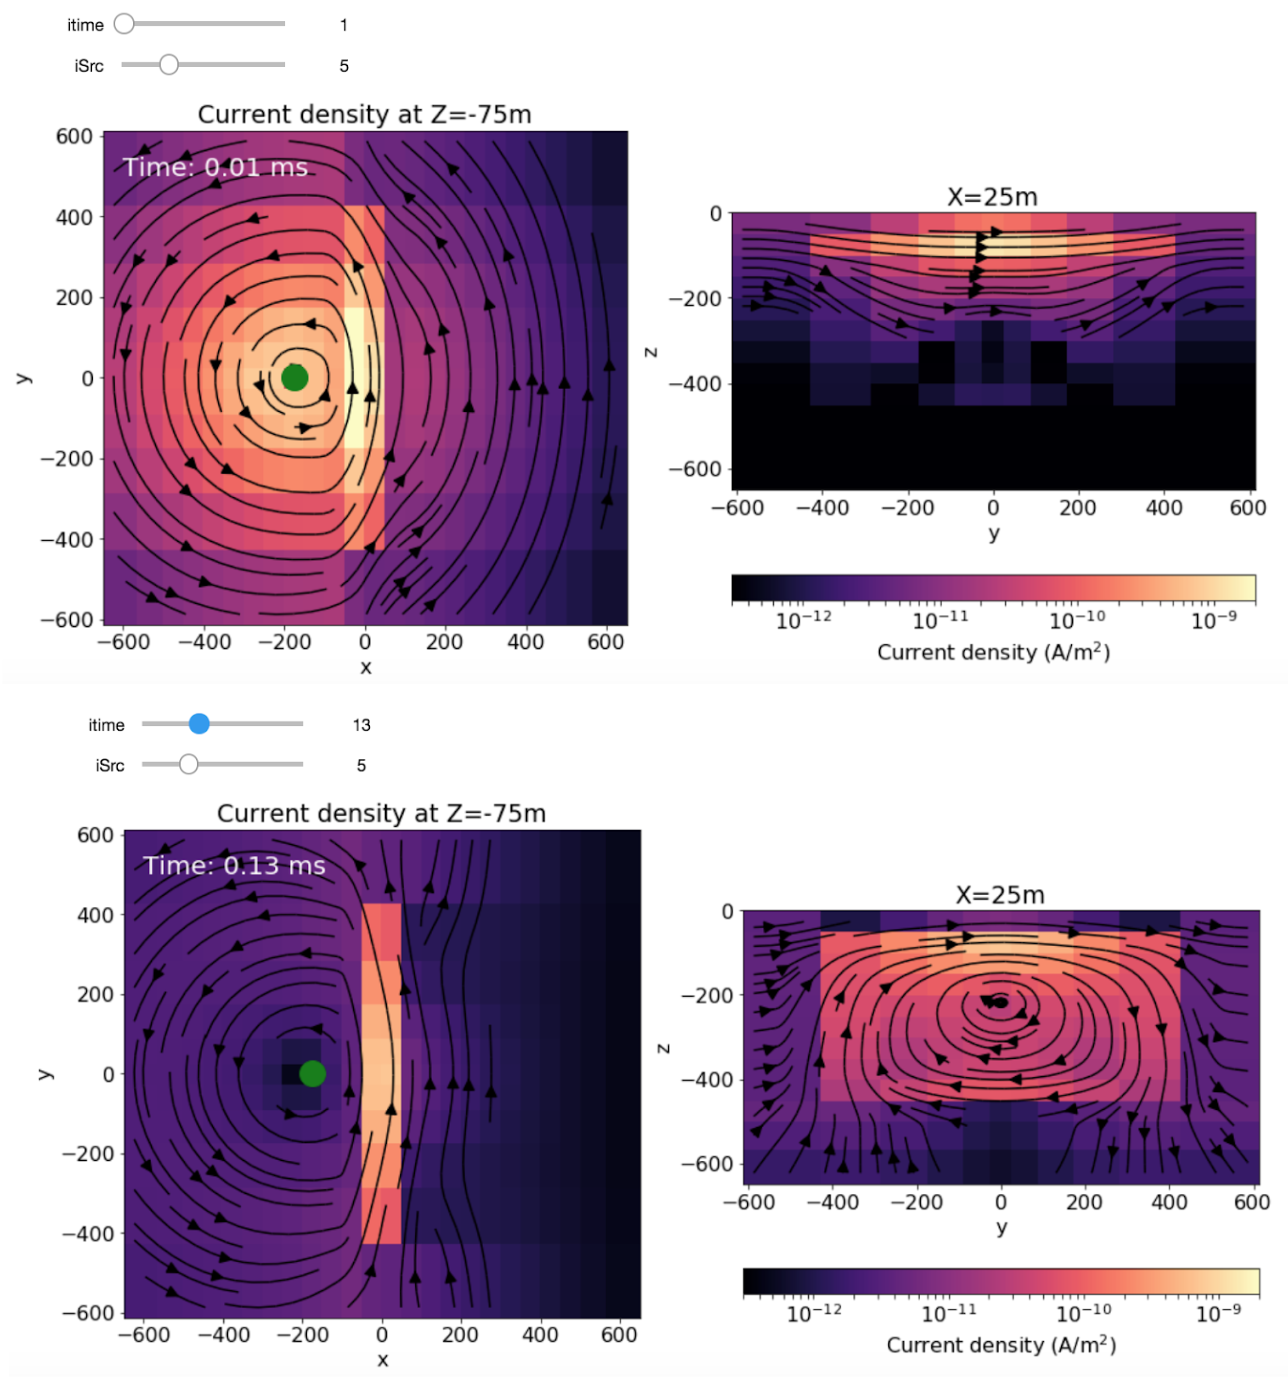
\includegraphics[width=0.8\columnwidth]{figures/currents-widget.png}
    \end{center}
\caption{
    Snapshot of widgets in the Jupyter environment that a select a time and source location for which to view the currents. Here, we show the current density at 0.01 ms (top) and 0.13 ms (bottom) after shut-off. The panel on the left shows a depth slice and the panel on the right shows a cross-section. The green dot indicates the source location.
}
\label{fig:currents-widget}
\end{figure}

